\documentclass[aspectratio=169,10pt]{beamer}
\usetheme{default}
\usecolortheme{seahorse}
\setbeamertemplate{navigation symbols}{}
\setbeamertemplate{footline}[frame number]
\usepackage{graphicx, booktabs, siunitx}
\graphicspath{{../figures/}}

\definecolor{sigcol}{HTML}{c2410c}
\definecolor{sbcol}{HTML}{1d4ed8}

\title{The Sideband Subtraction, Step by Step}
\subtitle{How wall--plastic coincidences become clean SiPM-wall MIP peaks \\
          n\_TOF EAR2 X17 --- run 224404}
\author{Dylan Neff \\[0.5ex] {\small analysis and slides prepared with Claude (Anthropic AI assistant)}}
\date{July 17, 2026}

\begin{document}

\begin{frame}\titlepage\end{frame}

% ---------------------------------------------------------------- idea
\begin{frame}{The problem the subtraction solves}
\begin{columns}
\column{.55\textwidth}
\begin{itemize}
\item In every bunch, wall hits and plastic hits also line up \emph{by chance}
      (pile-up), not just from real through-going particles.
\item These \alert{accidental} pairs fall inside the coincidence time window too,
      and they pollute the amplitude spectrum at low amplitude.
\item \textbf{Idea:} the accidentals are \emph{flat in time} --- so measure their
      amplitude shape in an off-peak \textbf{sideband}, scale it to the width of
      the signal window, and subtract.
\end{itemize}
\column{.45\textwidth}
\centering
\textcolor{sigcol}{\textbf{signal window}} $=$ MIP $+$ accidentals\\[1ex]
\textcolor{sbcol}{\textbf{sideband}} $=$ accidentals only\\[1ex]
\rule{0.8\textwidth}{0.4pt}\\[1ex]
true coincidences\\
$=\ \text{signal} - \dfrac{16\,\text{ns}}{100\,\text{ns}}\times\text{sideband}$
\end{columns}
\vskip1ex
{\footnotesize All plots below: one representative channel \textbf{WALB6}, high-purity
sample (post-recovery bunches, plastic hits $>$0.1 ms after the $\gamma$-flash).}
\end{frame}

% ---------------------------------------------------------------- step 1
\begin{frame}{Step 1 --- the two time windows}
\centering
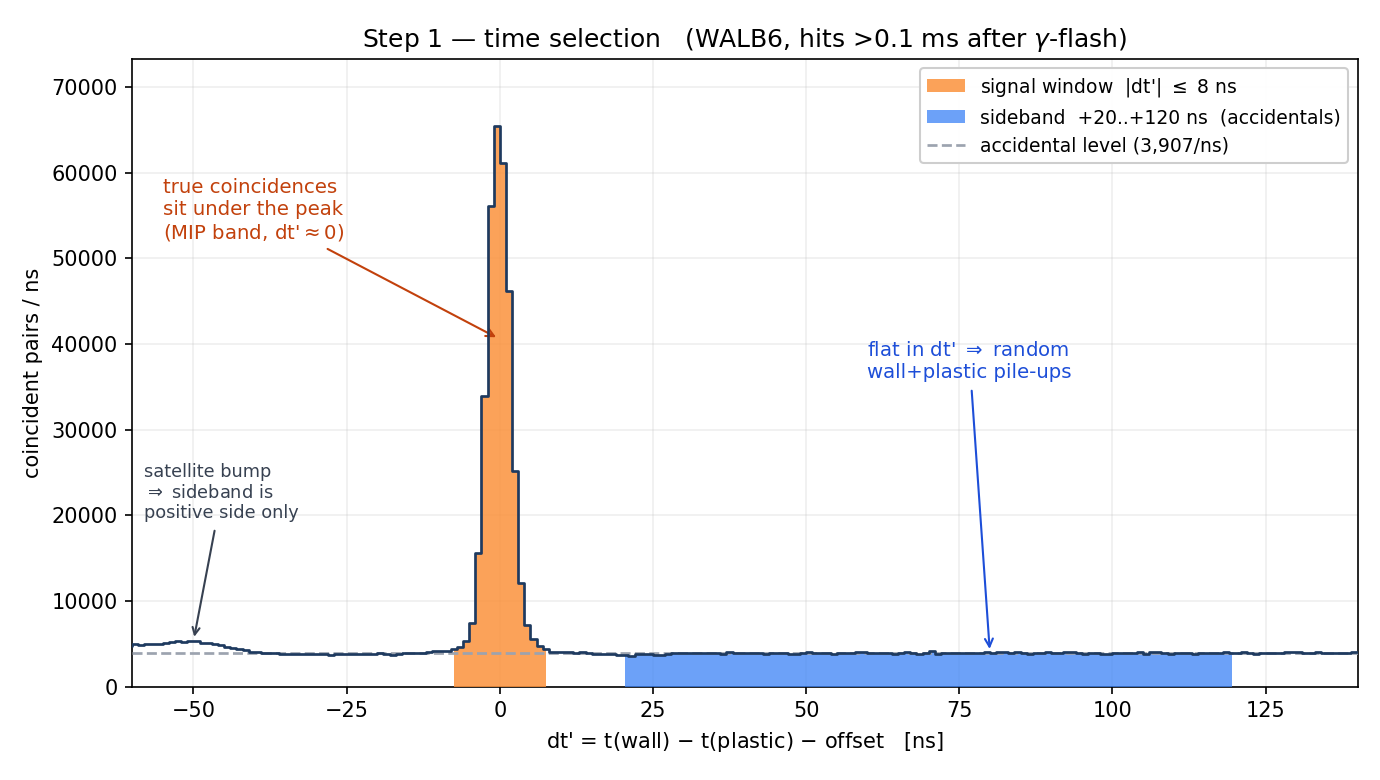
\includegraphics[height=.74\textheight]{15_pipeline/step1_time.png}\\
{\footnotesize After subtracting the per-channel offset, real pairs peak at
$\mathrm{dt}'=0$. \textcolor{sigcol}{Signal: $|\mathrm{dt}'|\le 8$ ns}.
\textcolor{sbcol}{Sideband: $+20$ to $+120$ ns} --- positive side only, to dodge
the $-50$ ns satellite bump. The sideband floor \emph{is} the accidental rate.}
\end{frame}

% ---------------------------------------------------------------- step 2
\begin{frame}{Step 2 --- amplitude spectrum inside the signal window}
\centering
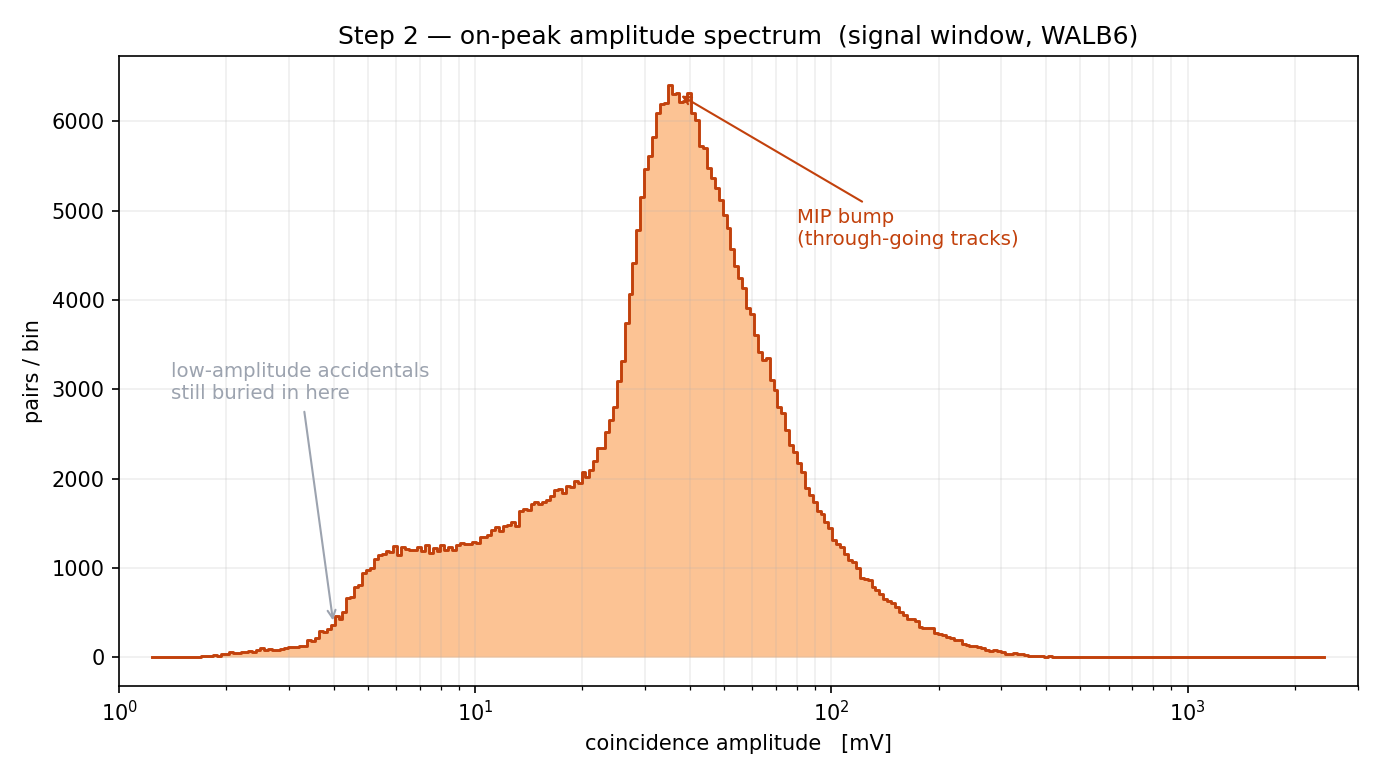
\includegraphics[height=.74\textheight]{15_pipeline/step2_signal.png}\\
{\footnotesize This is what you get with a plain time cut: a clear MIP bump near
35 mV, \emph{but} sitting on a large low-amplitude tail of accidental pairs. Not
yet a calibration-grade peak.}
\end{frame}

% ---------------------------------------------------------------- step 3
\begin{frame}{Step 3 --- the sideband is the accidental shape}
\centering
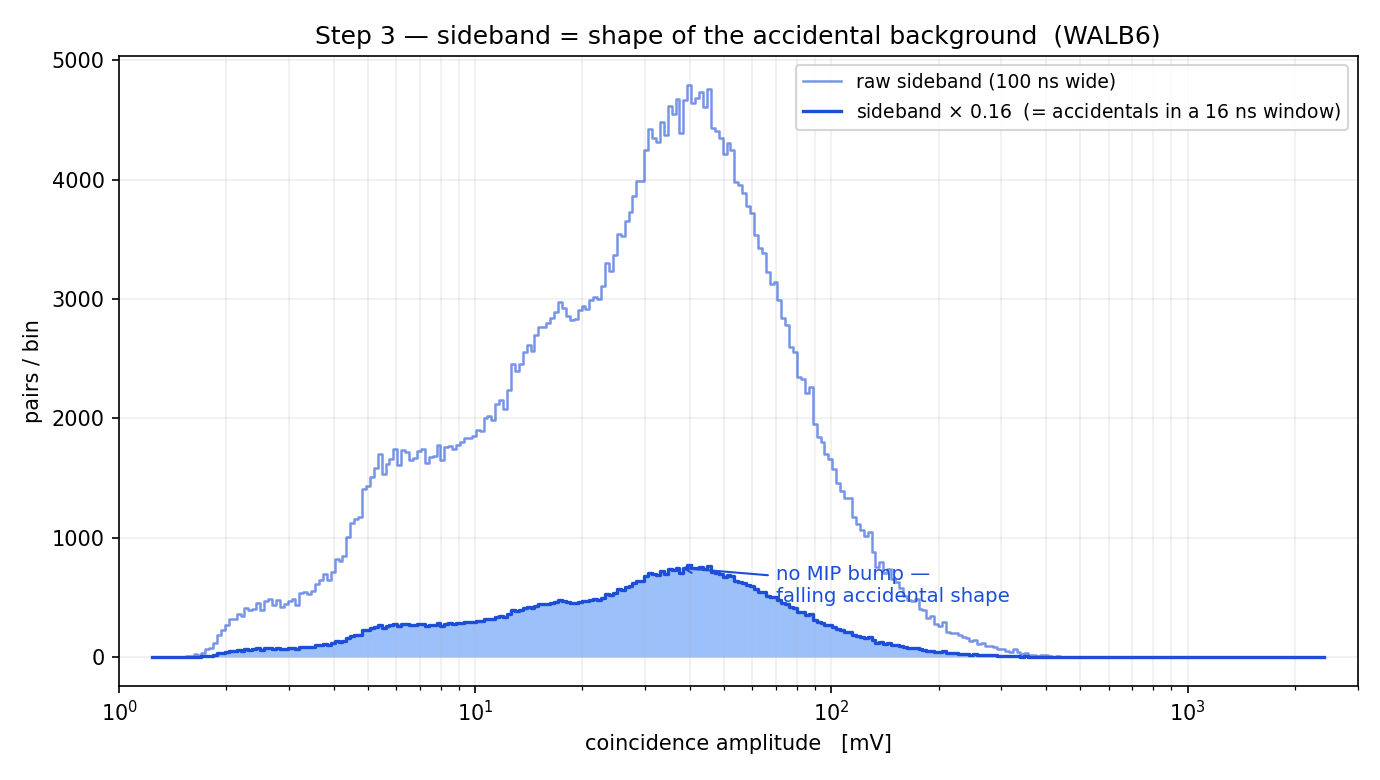
\includegraphics[height=.74\textheight]{15_pipeline/step3_sideband.png}\\
{\footnotesize Same pairs, but from the off-peak window: \textbf{no MIP bump} ---
just the falling accidental amplitude shape. Scaling by $16/100$ converts the
100 ns-wide sideband into the accidental content expected inside the 16 ns-wide
signal window.}
\end{frame}

% ---------------------------------------------------------------- step 4
\begin{frame}{Step 4 --- overlay: same accidental floor}
\centering
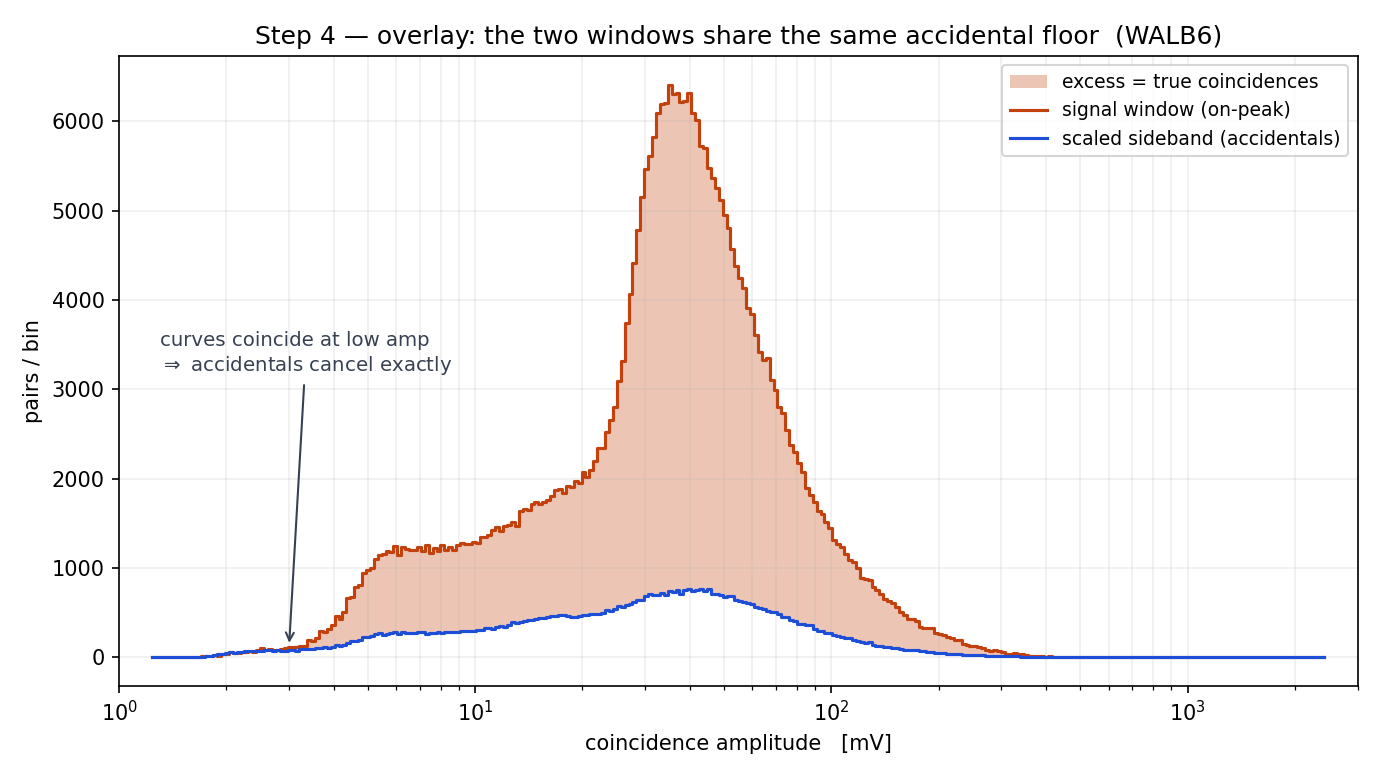
\includegraphics[height=.74\textheight]{15_pipeline/step4_overlay.png}\\
{\footnotesize The two curves lie on top of each other at low amplitude --- the
accidentals are identical --- and separate only where the real MIP population
lives. The \textcolor{sigcol}{shaded gap} is the true-coincidence excess.}
\end{frame}

% ---------------------------------------------------------------- step 5
\begin{frame}{Step 5 --- subtract $\Rightarrow$ clean MIP peak}
\centering
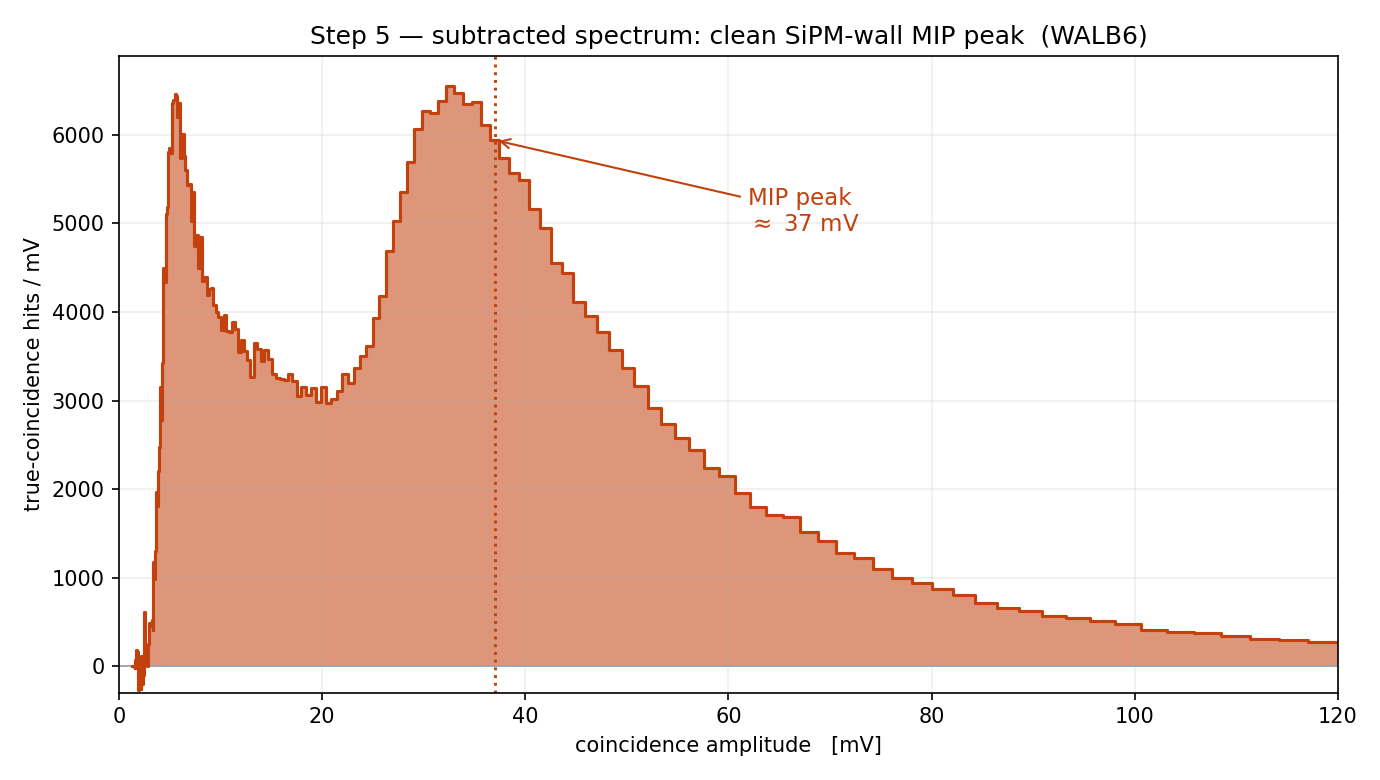
\includegraphics[height=.74\textheight]{15_pipeline/step5_subtracted.png}\\
{\footnotesize $\text{signal} - 0.16\times\text{sideband}$: the accidental tail
cancels and a clean SiPM-wall MIP peak at $\approx 37$ mV remains --- this is the
per-channel calibration landmark. (The narrow $\sim$5 mV feature is a real
low-amplitude coincidence population, present in all arms.)}
\end{frame}

% ---------------------------------------------------------------- overview
\begin{frame}{The whole pipeline on one slide (WALB6)}
\centering
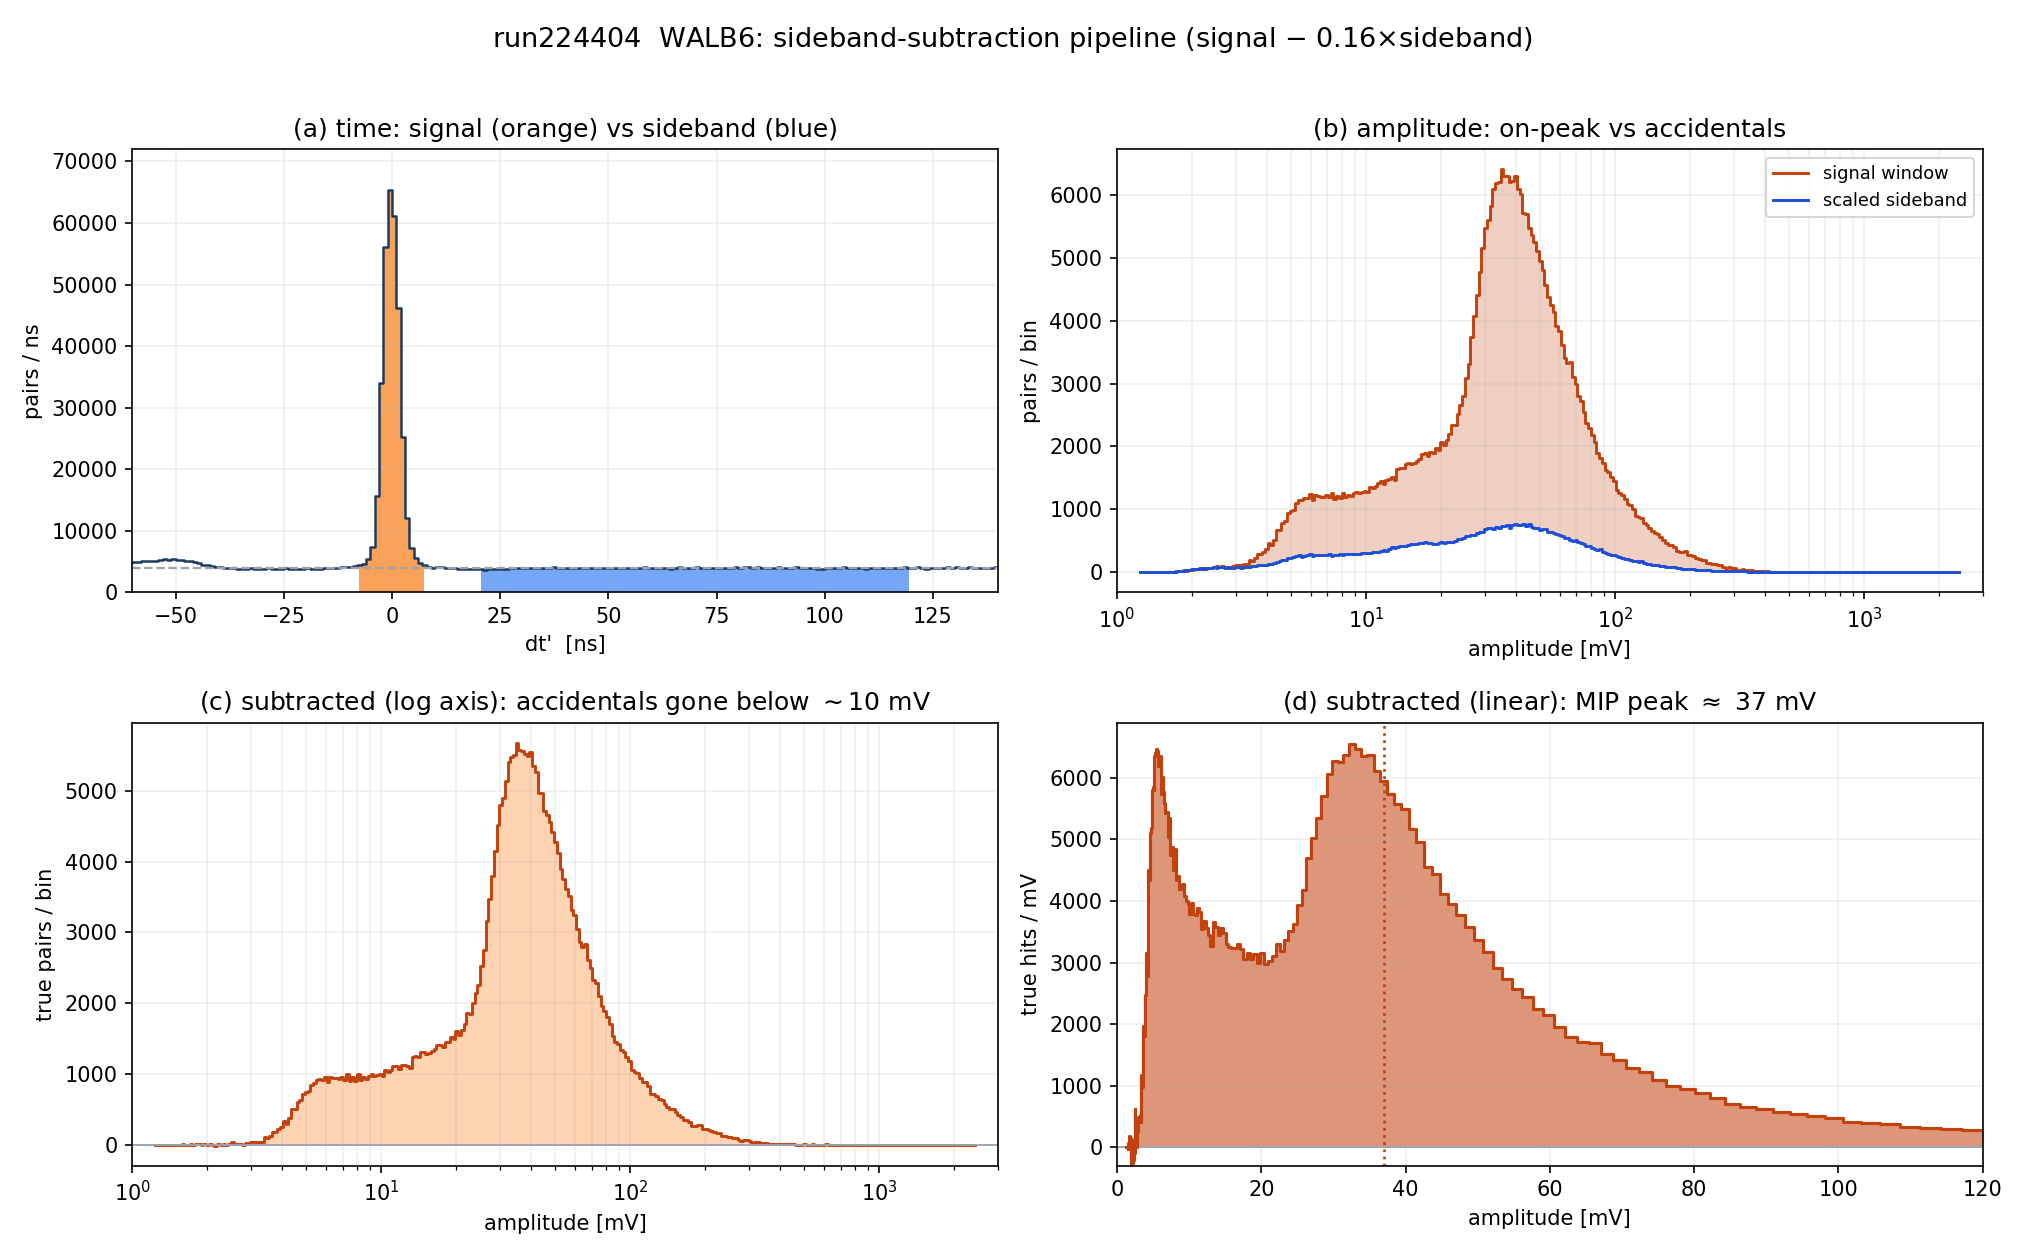
\includegraphics[height=.80\textheight]{15_pipeline/pipeline_overview.png}
\end{frame}

% ---------------------------------------------------------------- null test
\begin{frame}{Sanity check: subtraction cannot manufacture a peak}
\centering
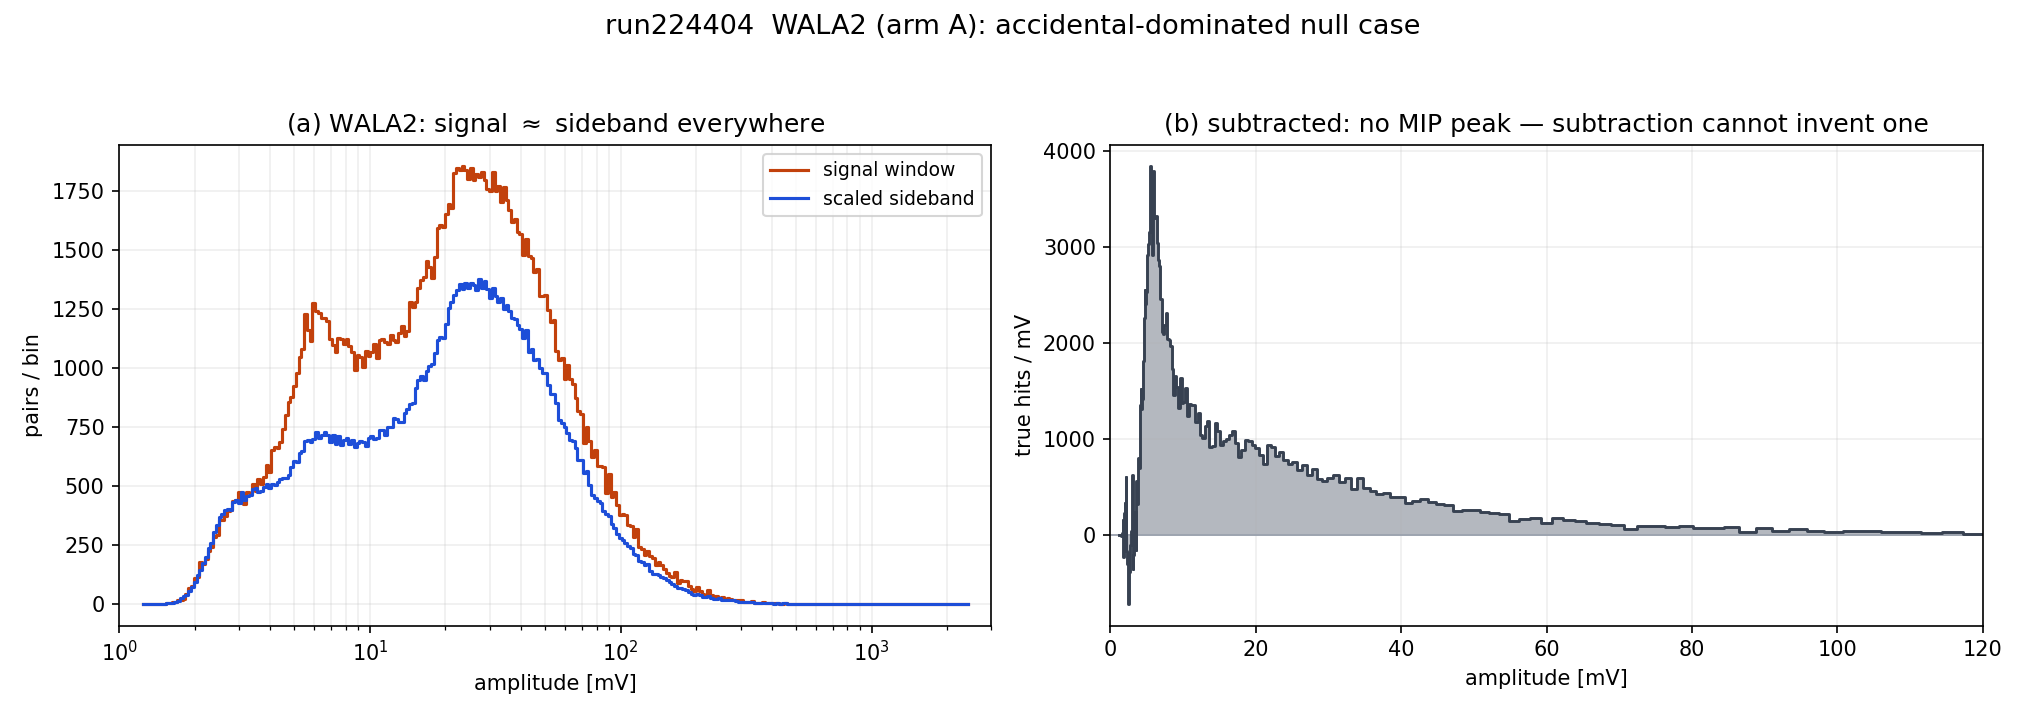
\includegraphics[width=.96\textwidth]{15_pipeline/null_contrast.png}\\
{\footnotesize Arm-A channel WALA2: here the signal window is accidental-dominated,
so signal and scaled sideband have the \emph{same} shape. After subtraction the
residual just falls off --- \textbf{no fake MIP peak}. The method only reveals a
peak where a real one exists (arms B/C), never invents one.}
\end{frame}

% ---------------------------------------------------------------- generalizes
\begin{frame}{Same recipe, all 16 B/C channels}
\centering
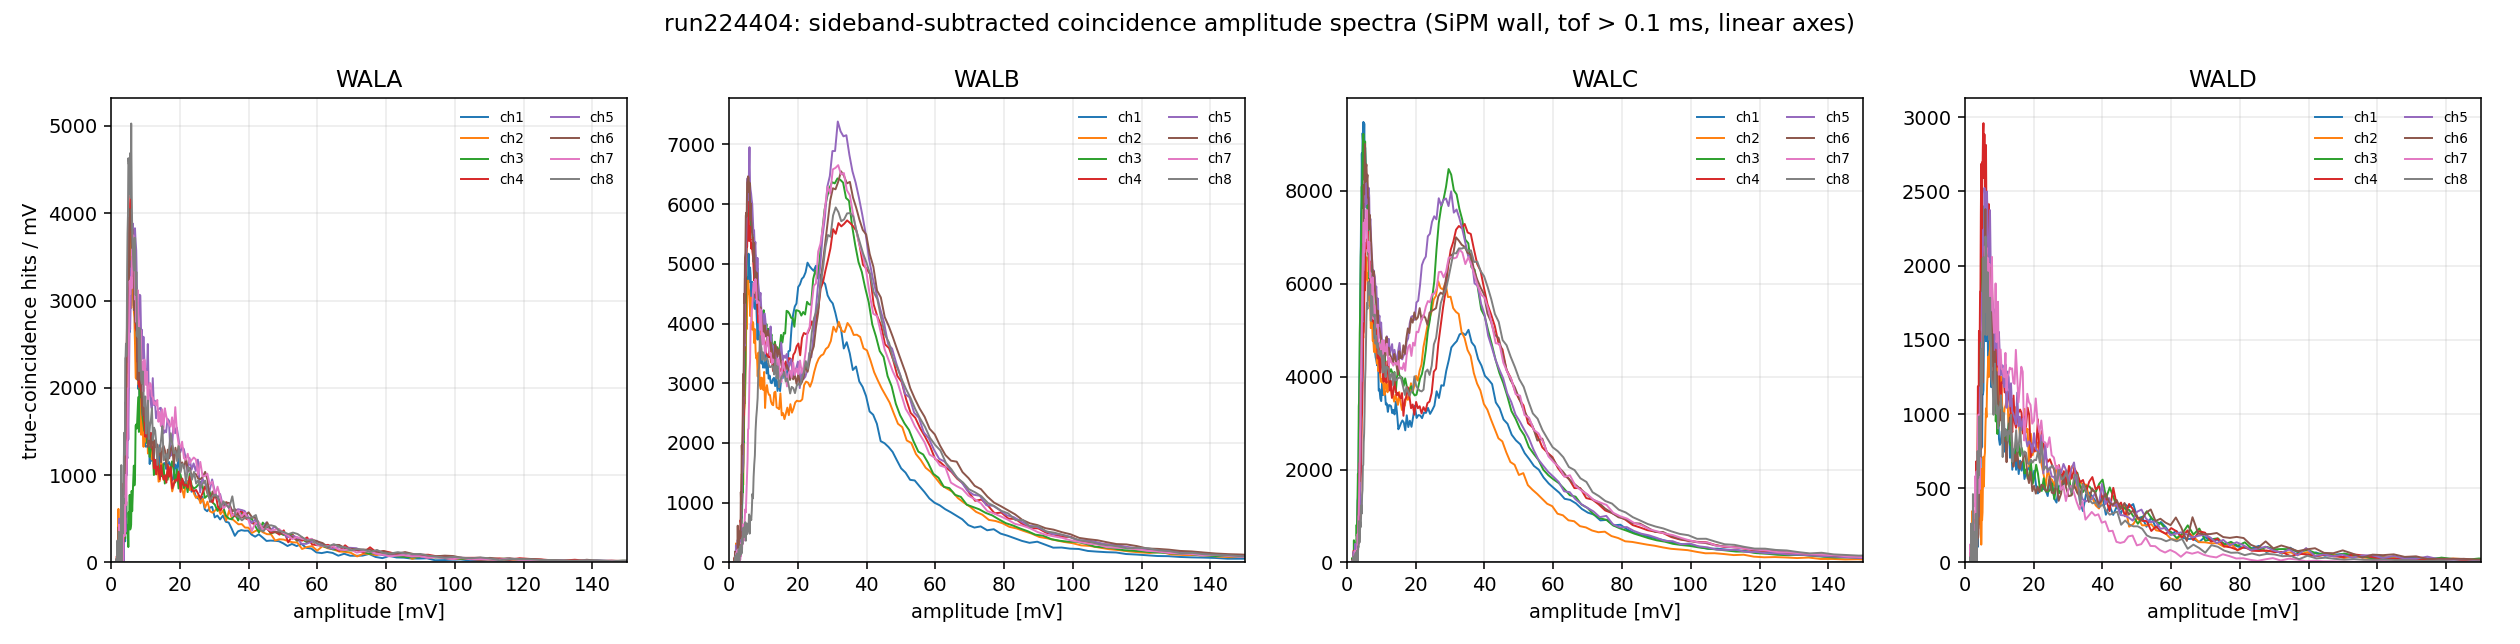
\includegraphics[width=\textwidth]{06_07_geometry_mip/mip_wall_spectra_linear.png}\\
{\footnotesize Each curve is one wall channel's subtracted spectrum. \textbf{B/C:
clean MIP peaks 29--39 mV on all 16 channels} $\Rightarrow$ per-channel gain
landmark. A/D: accidental-dominated (null case above), MIP cause still open.}
\end{frame}

\begin{frame}{Summary}
\begin{itemize}
\item The ``nice'' MIP peaks are \textbf{not} the raw in-time spectrum --- they are
      $\text{signal} - 0.16\times\text{sideband}$.
\item \textcolor{sigcol}{Signal} $= |\mathrm{dt}'|\le 8$ ns (MIP $+$ accidentals);
      \textcolor{sbcol}{sideband} $= +20$ to $+120$ ns (accidentals only), scaled
      by the window-width ratio $16/100 = 0.16$.
\item The subtraction removes the low-amplitude accidental tail exactly, leaving a
      calibration-grade SiPM-wall MIP peak wherever real through-going tracks exist.
\item Verified null: where there is no MIP population, the subtraction returns no
      peak.
\end{itemize}
\end{frame}

\end{document}
